\chapter{Ergebnisse}

- bleibt der charakter stehen, sieht die aimation etwas komsich aus. dafür mehr responsive als wenn er zurück oder weiter steppen würde
- je nachdem wann input gepollt wird kann erster schritt oft sehr klein sein

\section{Limitierungen}

\begin{figure}
    \centering
    \begin{subfigure}[t]{.4\linewidth}
        \centering
        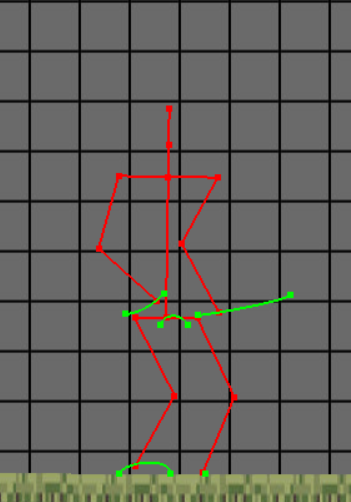
\includegraphics[width=0.75\linewidth]{images/even_ground_slow.png}
        \caption{Gehen auf ebenem Untergrund.}
        \label{even_slow}
    \end{subfigure}
    \begin{subfigure}[t]{.4\linewidth}
        \centering
        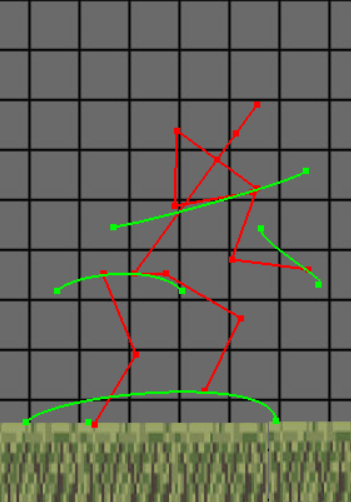
\includegraphics[width=0.75\linewidth]{images/even_ground_fast2.png}
        \caption{Rennen auf ebenem Untergrund.}
        \label{even_fast}
    \end{subfigure}
    \begin{subfigure}[t]{.4\linewidth}
        \centering
        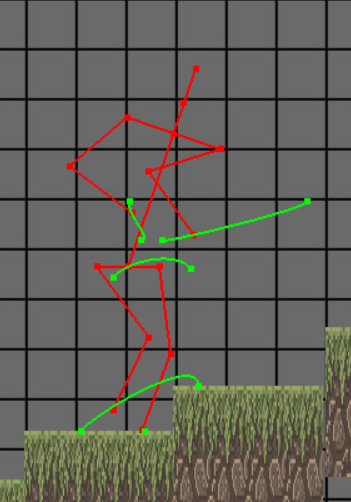
\includegraphics[width=0.75\linewidth]{images/going_up3.png}
        \caption{Bewegung bergauf.}
        \label{uphill}
    \end{subfigure}
    \begin{subfigure}[t]{.4\linewidth}
        \centering
        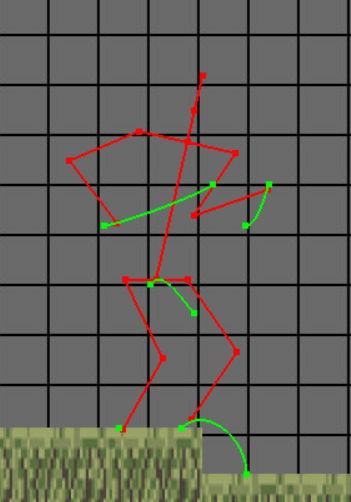
\includegraphics[width=0.75\linewidth]{images/going_down1.png}
        \caption{Bewegung bergab.}
        \label{downhill}
    \end{subfigure}
    \begin{subfigure}[t]{.4\linewidth}
        \centering
        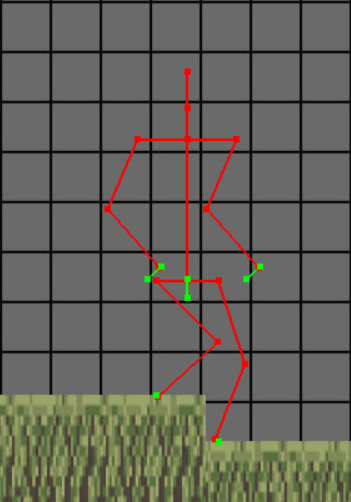
\includegraphics[width=0.75\linewidth]{images/standing_uneven.png}
        \caption{Stehen auf unebenem Untergrund.}
        \label{standing_uneven}
    \end{subfigure}
    \begin{subfigure}[t]{.4\linewidth}
        \centering
        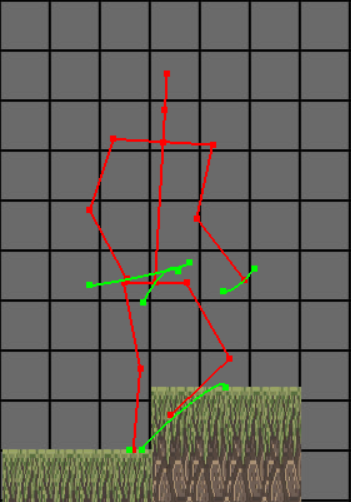
\includegraphics[width=0.75\linewidth]{images/clip_through_gorund.png}
        \caption{Ein Bein bewegt sich beim aufwärts gehen durch den Boden.}
        \label{clip_through_ground}
    \end{subfigure}
    \caption{Beispiele generierter Animationen. Das Skelett ist in rot dargestellt. Die grünen Linien stellen die Splines dar, an denen sich die entsprechenden Knochen entlang bewegen.}
\end{figure}